\section{2020/01/08 - Introduction}

\begin{definition}
    Let $x, y \in \R^n$, $0 \leq \lambda \leq 1$, $z(\lambda) = \lambda x + (1 - \lambda)y$ is a \underline{convex combination} of $x$ and $y$
\end{definition}

This simple definition leads to many strong algebraic and topological results.

For this course, we will work in Euclidean space $\E^n$ with inner product $\langle x, y \rangle$ and norm $||x|| = \sqrt{\langle x, y \rangle}$.

On $\R^n$, we will use the familiar dot product $\langle x, y \rangle = x^\intercal y = \sum_{i = 1}^n x_iy_i$ and norm $||x|| = \sqrt{\sum_{i=1}^n x_i^2}$.

\begin{definition}
    $C \subseteq \E^n$ is \underline{convex set} if $x, y \in C \ 0 \leq \lambda \leq 1 \Rightarrow \lambda x + (1- \lambda)y \in C$ (or equivalently, $x, y \in C \Rightarrow [x,y] \subseteq C$)
\end{definition}

\begin{note} We can write $z(\lambda)$ in the following ways:
    \begin{align*}
        z(\lambda) &= \lambda x + (1 - \lambda) y \\
        &= y + \lambda (x - y) \\
        &= x + (1 - \lambda)(y - x)
    \end{align*}
\
    The second equation can be interpreted as: ``Beginning at $y$ and moving towards $x$''. And, the third equation can be interpreted as: ``Beginning at $x$ and moving towards $y$''
\end{note}

\begin{definition}
    Let $C \subseteq \E^n$, $C$ convex set. Then $f: C \rightarrow \R$ is a \underline{convex function} if:
    \begin{equation*}
        f(\lambda x + (1 - \lambda) y) \leq \lambda f(x) + (1 - \lambda)f(y)
    \end{equation*}
    $\forall x, y \in C, \ \forall 0 \leq \lambda \leq 1$
\end{definition}

\begin{example}
    ~\\
    \begin{minipage}{\textwidth}
        \centering
        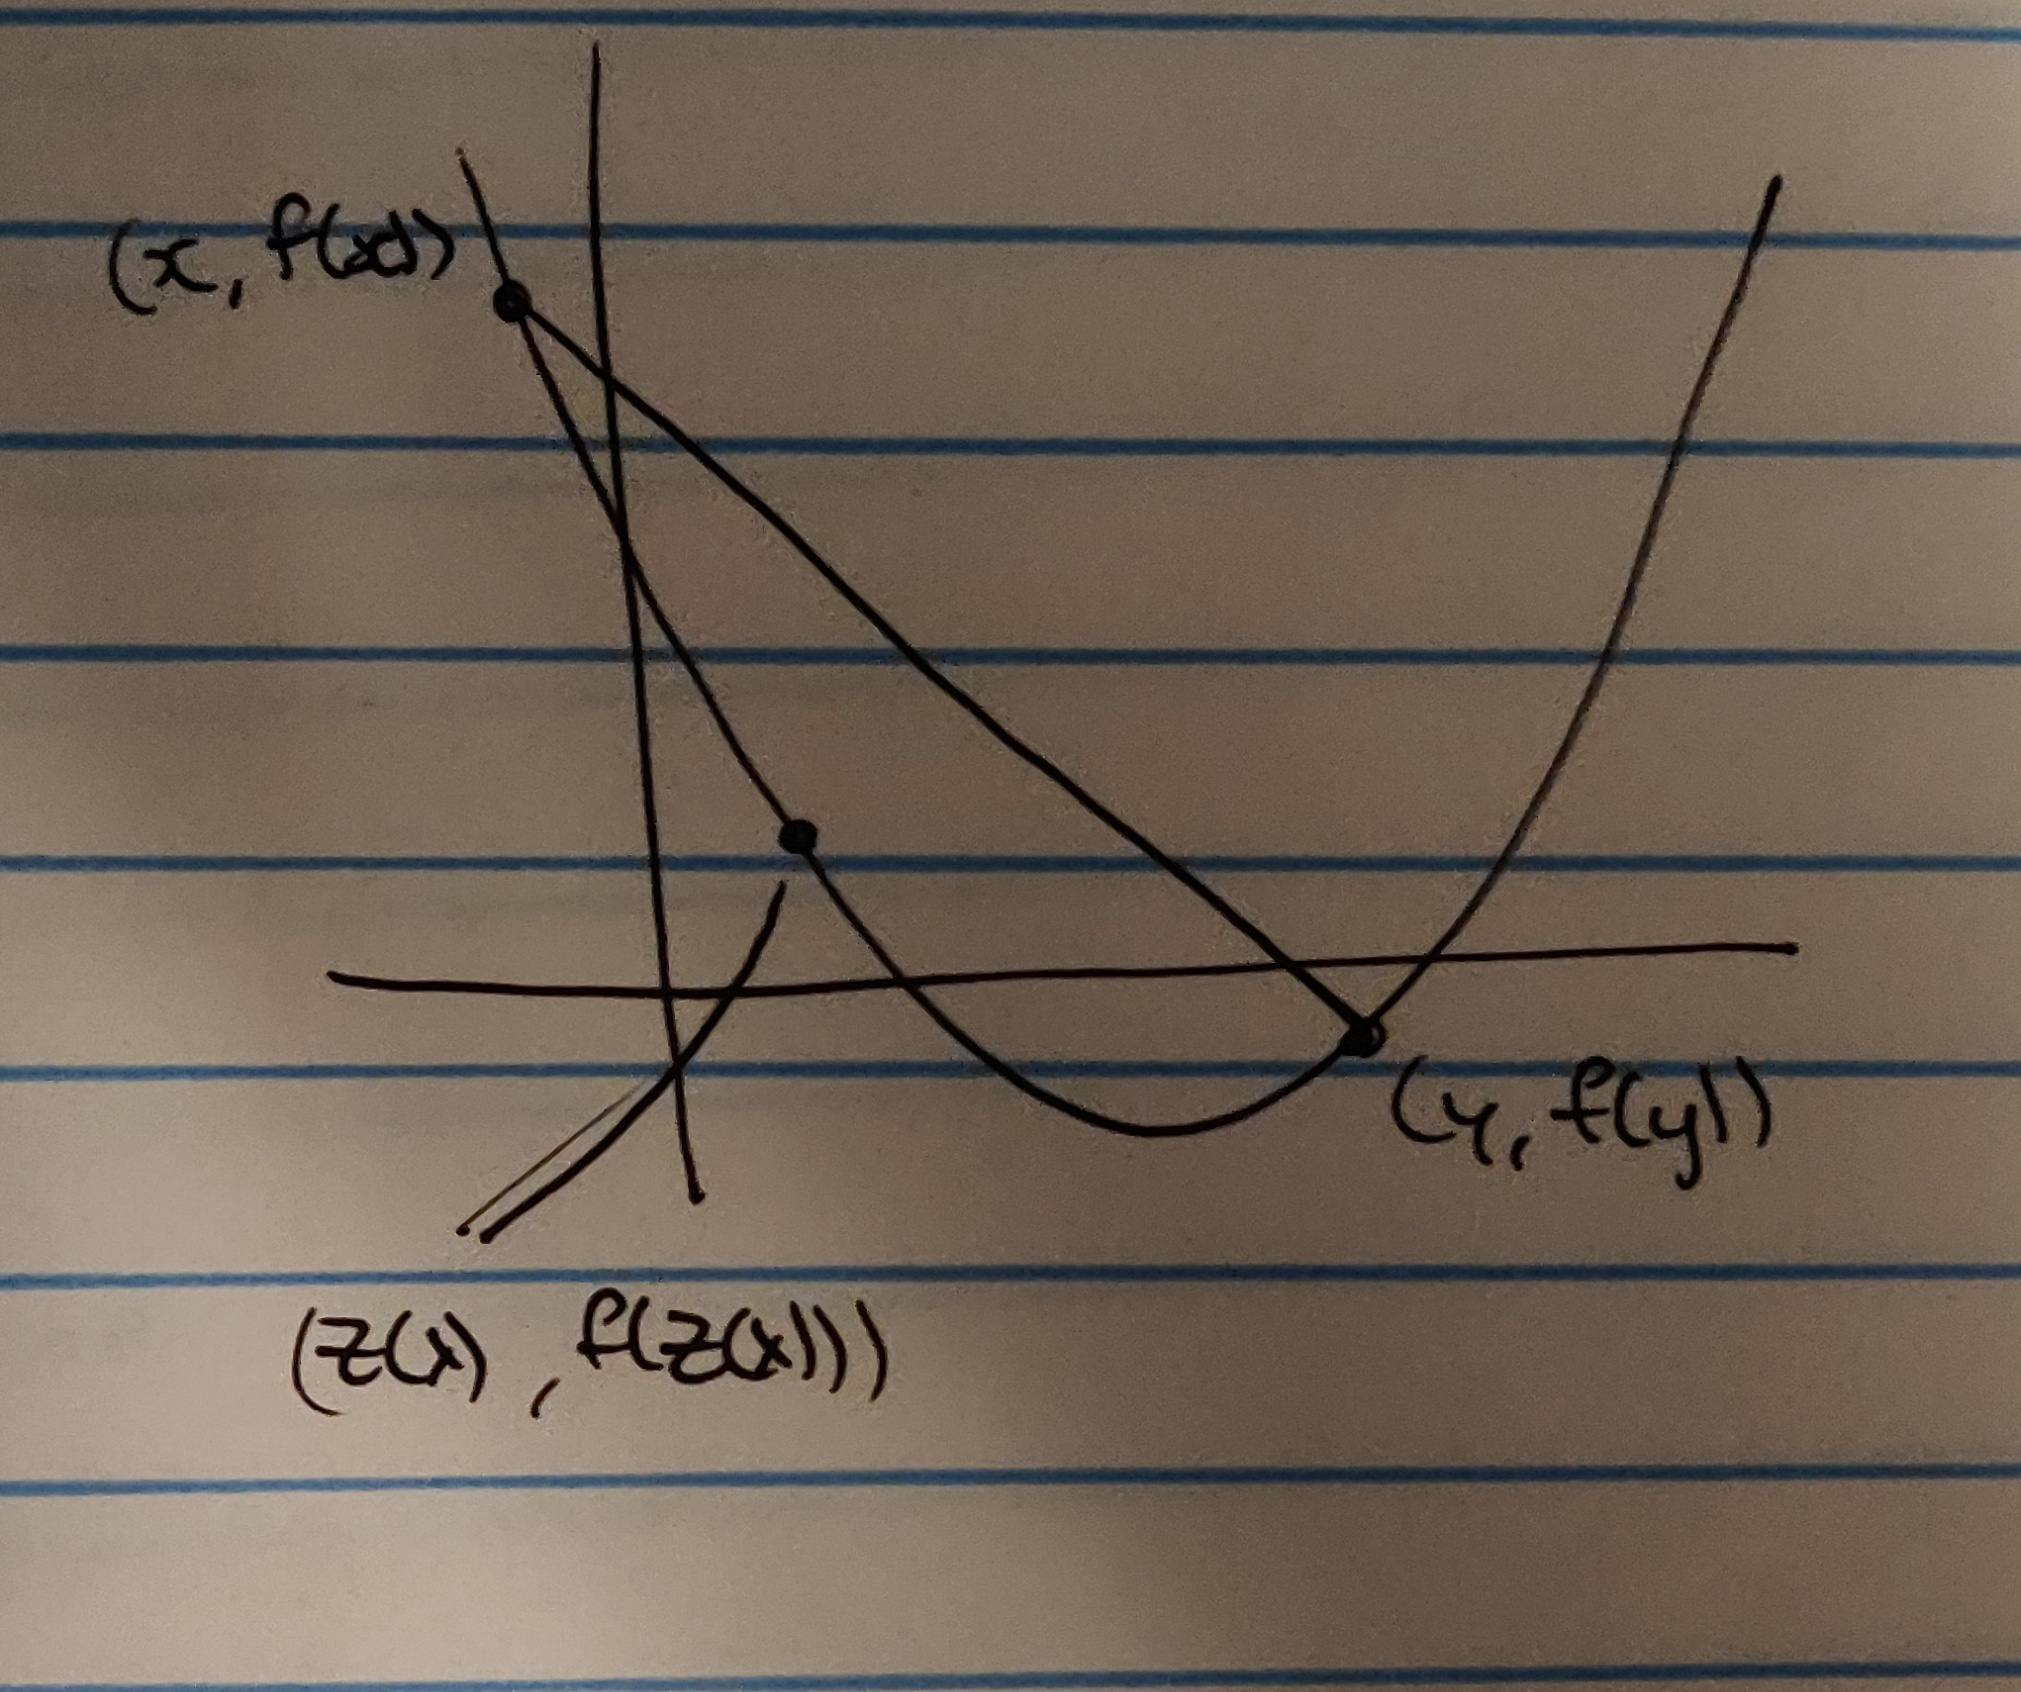
\includegraphics[width=0.5\textwidth]{images/co463/lec1-convex-function}
        \captionof*{figure}{The line between $(x, f(x))$ and $(y, f(y))$ is called the \underline{secant line}. For convex function, the graph lies \underline{below} the secant line.}
    \end{minipage}
\end{example}

The region \underline{above} the graph is called the \underline{epigraph}, denoted $\epi f$.
It is defined as:
\begin{equation*}
    \epi f = \{ (r, x) \in \R \times \E^n\::\:x \in C, f(x) \subseteq r\}
\end{equation*}
for $f: C \rightarrow \R$, $C$ convex.

We will see that:
\begin{theorem}
    $f$ is a convex function if and only if $\epi f$ is a convex set
\end{theorem}

Suppose we have the following minization problem:
\begin{align*}
    p^* = &\min f(x) \\
    &\text{s.t} \ x \in C
\end{align*}
where $C \in \E^n$ convex, $f:C \rightarrow \R^n$ convex function.

We will show that: $f$ convex $\Rightarrow$ (local min \underline{iff} global min)

\underline{Applications:}

\begin{itemize}
    \item Linear Programming
    \item Convex Relaxation
\end{itemize}

\clearpage